\section{Côte du sud}

Date: 20/10/2009

\begin{multicols}{2}

Bonjour,

Alors alors, par où commencer... Ah oui, par le premier jour..

Nous sommes lundi 12, je suis à l'heure a l'aéroport, mon avion est à l'heure lui aussi, je demande confirmation pour savoir si l'arrière de l'appareil dessert bien Miami lui aussi comme il est indiqué à l'avant :), et c'est parti pour un survol de l'atlantique, 10h de vol, 12h de transit forcé sur le sol Américain car l'aeéoport n'a pas de zone internationale, je vais voir la plage, me balade dans Miami, sympa cette escale..

\hspace*{-0.65cm}
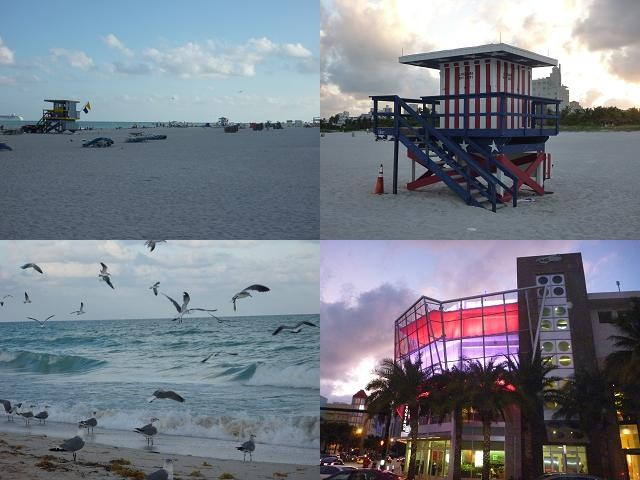
\includegraphics[width=4.8cm]{articles/Cote-du-sud/1255996649K0tQ.jpg}
Miami beach.

Puis c'est reparti pour 6 heures de vol direction Lima, capitale du Perou, la je decouvre une ville immense (8 million d'habitants) aux différents quartiers très différents. Du quartier très pauvre où me laisse le collectivo (minivan transformé en minibus très cheap).

\hspace*{-0.65cm}
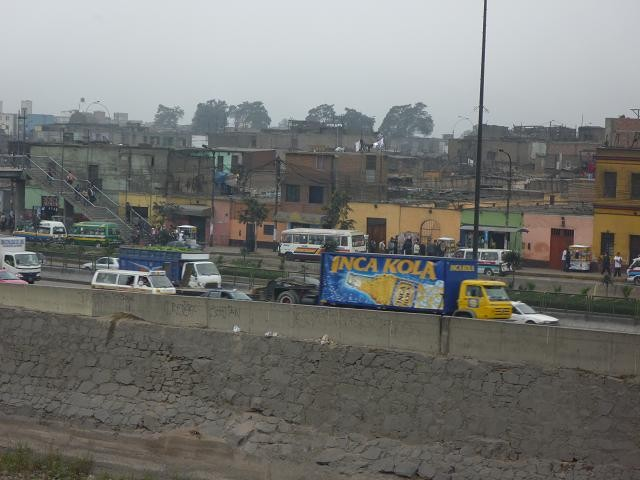
\includegraphics[width=4.8cm]{articles/Cote-du-sud/1255996655Vfsf.jpg}
Quartier pauvre de Lima.

Au quartier déjà un peu plus riche autour de la Plaza de Armas, ici une photo d'une bâtiment du gouvernement qui borde la Plaza de Armas. Je découvrirais plus tard que chaque ville comporte une place de ce nom, et il s'agit en général d'une place richement décorée, contrastant avec les alentours.

\hspace*{-0.65cm}
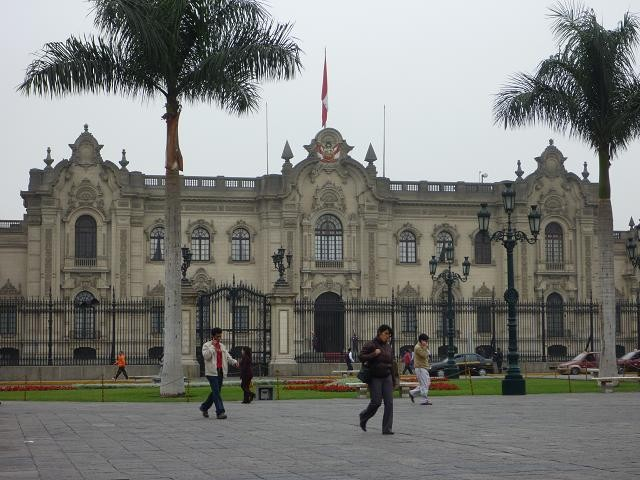
\includegraphics[width=4.8cm]{articles/Cote-du-sud/1255996660JAoN.jpg}
Plaza de Armas.

Reprenons le fil des choses, je suis arrivé à 4h30 du matin et j'ai attendu un peu le jour avant de sortir de l'aéroport, j'ai eu le temps de me renseigner comment éviter les taxi hors de prix puis me voila avec mon sac dans un collectivo bondé direction le centre de Lima, il me dépose un peu  à l'extérieur où vous avez pu voir le Lima mal famé, puis je marche vers la place des armes où je vais me renseigner à l'office du tourisme pour des bus en direction du Sud, vers Pisco où il y a de belle choses à voir lorsqu'on a le pied marin. Des bus partent toutes les 8 minutes, c'est presque trop facile... Je passe le reste de la matinée à me ballader dans Miraflorès, quartier chic de Lima (tout est relatif) au bord de la falaise qui donne sur l'océan, puis je prend mon bus pour Pisco. Je visiterai plus en détail Lima à mon retour avant de revenir sur le vieux continent.

\hspace*{-0.65cm}
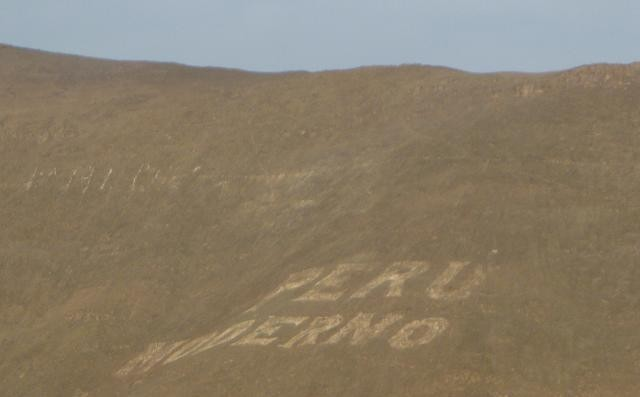
\includegraphics[width=4.8cm]{articles/Cote-du-sud/1255996643RUpx.jpg}
Peru moderno.


Pisco, ville touchée par un séisme deux ans plus tôt, tout est en reconstruction, on sent vraiment la pauvreté ici. Le Lonely Planet me dit de me méfier, l'hôtel me dit de sortir sans sac, de cacher mon appareil photo et de laisser mon passeport dans le coffre fort de la chambre (pourtant j'avais pris une chambre sans option, le coffre est de serie, ça laisse présager..). Quoi de mieux pour faire flipper le voyageur en visite ? Je ne me suis jamais senti en insécurite à Pisco, les gens sont sympa, l'extrême pauvreté alliée à l'aridité du sol donne à la ville un caractère étrange.

\hspace*{-0.65cm}
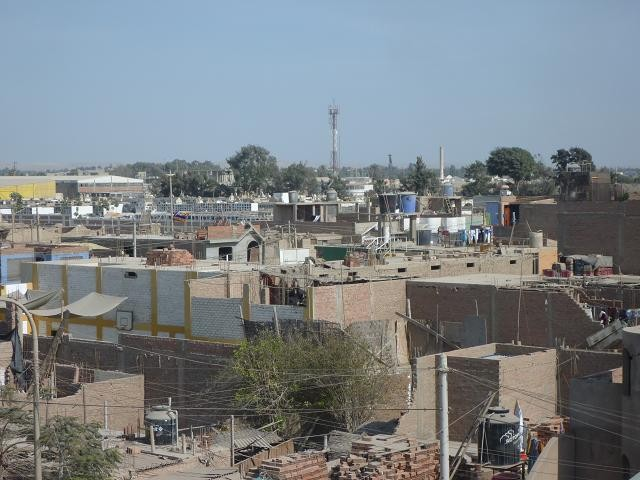
\includegraphics[width=4.8cm]{articles/Cote-du-sud/12559974777RC0.jpg}
Pisco.


Allez, une petite photo d'un étalage, parce que vous le valez bien.

\hspace*{-0.65cm}
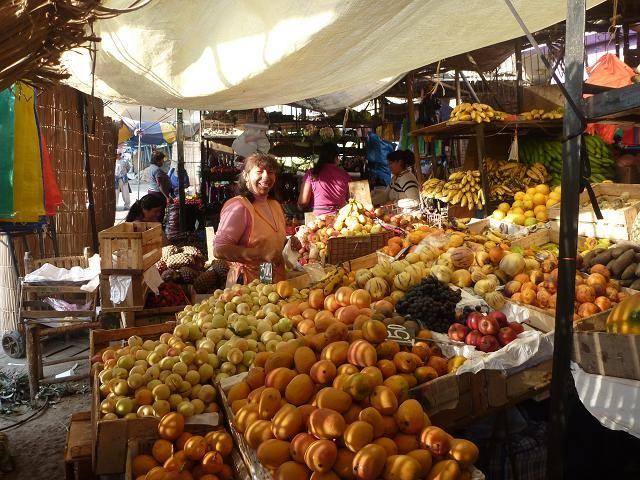
\includegraphics[width=4.8cm]{articles/Cote-du-sud/1255997490cIfD.jpg}
Marché de Pisco.


Heureusement pour les Piscoñeros, une belle richesse est aux portes de la ville, il s'agit des iles Balestas, véritable condensé de faune (pas très) sauvage, ainsi qu'un mystère archéologique. Un chandelier a été tracé il y a des centaines d'années dans le sable sur le flanc d'une montagne, et l'énigme irrésolue est de savoir comment se fait il que le dessin ne s'efface pas. Nous voyons ce chandelier d'un bateau en allant voir les îles Balestas. Les deux théories étant que le dessin est sur une face sous le vent, donc protégée, et que la sédimentation aurait durci le sol. Quoiqu'il en soit il est interdit de débarquer pour aller vérifier.

\hspace*{-0.65cm}
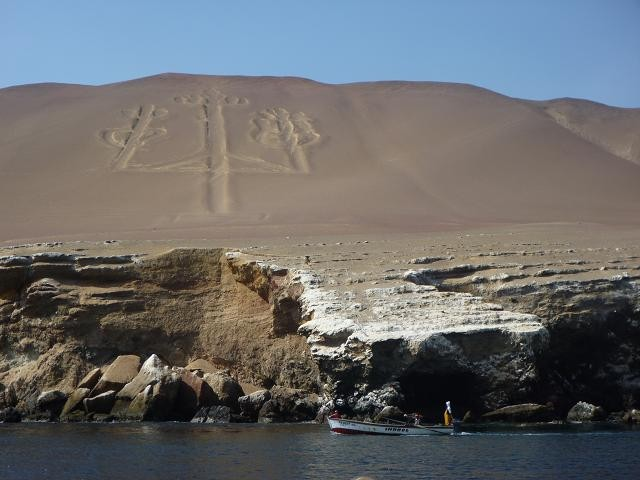
\includegraphics[width=4.8cm]{articles/Cote-du-sud/1255997496rIn7.jpg}
Chandelier de Paracas.


Et nous voici sur les îles, ici vit un grand nombre de pélicans pingouins, lions des mers et plein d'autres oiseaux..

\hspace*{-0.65cm}
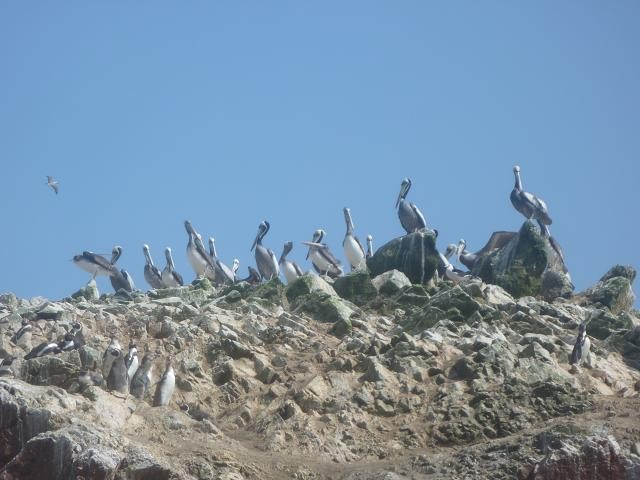
\includegraphics[width=4.8cm]{articles/Cote-du-sud/1255997482Hoy0.jpg}
Pélicans aux Balestas.


Regardez moi cette star...

\hspace*{-0.65cm}
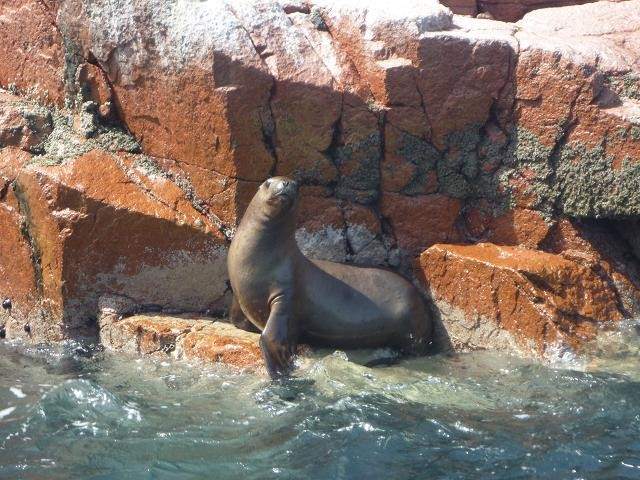
\includegraphics[width=4.8cm]{articles/Cote-du-sud/1255997520UtdU.jpg}
Who is the boss ?


Me voila reparti sur la route direction Ica, et surtout Huacachina, petit Oasis touristique au milieu des dunes pour faire du sandboard, activité vivement conseillée par mes très chères colocs qui l'ont pratiquée un an plus tôt et en ont encore le sourire aujourd'hui quand elles en parlent (Hélène et Dova, merci pour le conseil, je me suis régalé !!). Le concept ? Une oasis entourée de dunes qui sert de camp de base pour partir deux heures en areñeros, sorte 4*4 au design lunaire avec lequel on va à fond dans les dunes, dévalant les pentes et dérapant de partout, puis séance de sandboard, snowboard des sables. Et bien vous savez quoi ? on se dit que c'est facile quand on sait faire du snow, et en fait ça l'est pas tant que ça, mais bon j'ai quand même réussi à faire mes virages et quelques belles descentes.

Voici votre envoye special au debut du tour..

\hspace*{-0.65cm}
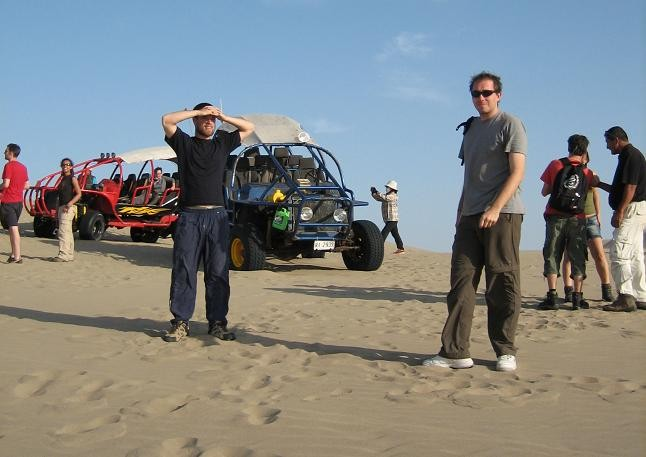
\includegraphics[width=4.8cm]{articles/Cote-du-sud/1255997503PLr1.jpg}
Areneros.


Pour le concept du sandboard, c'est par ici..

\hspace*{-0.65cm}
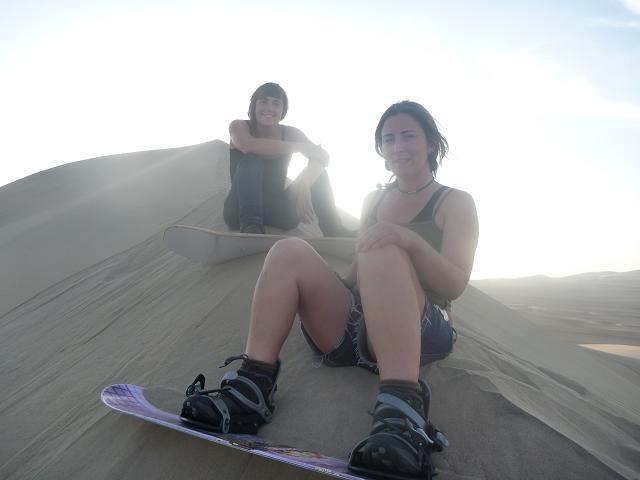
\includegraphics[width=4.8cm]{articles/Cote-du-sud/1255997499n41M.jpg}
Sandboard.


OK, c'est pas moi sur la planche, j'ai des videos de mes descentes mais il faudra attendre la fin du voyage pour les voir car elle demandent d'être travaillées pour être au bon format. Je rencontre plein de gens à Huacachina, dont deux Belges que vous pouvez voir sur les deux photos ci-dessus (Quentin a côté de moi et Maritv est la plus haute des deux sandboardeuses), une famille d'Américains qui a pris 11 mois pour voyager around ze world, avec deux ados, j'adore ce concept, et les parents sont bien sympas, on a discuté un long moment. Je croise aussi Didier au sandboard, on se reverra à Nazca.

Nazca, petite ville, grande énigme archéologique (encore une !). Nazca est proche de grands plateaux arrides sur lesquels une britanique, Maria Reiche, a découvert vers 1930 que des symboles géoemétriques, essentiellement des lignes parfaitement droites on été tracées en déplaçant simplement les pierres au sol. La encore on ne sait pas comment le phénomène ne s'efface pas avec le temps, un simple coup de vent devrait suffire, et pourtant.. La deuxième question est de savoir la signification de ces lignes, personne ne la connait, plusieurs théories ont été avancées suivant des modèles mathématiques, suivant les alignements des astres à certaines périodes de l'année.. Et la troisième question est de savoir comment cela a été fait. En effet il est indispensable d'avoir un point de vue du ciel pour faire ces dessins gigantesques, hors cela n'existait pas à l'époque. A ces lignes s'ajoutent un certain nombre de geoglyphes, dessins représentatifs d'animaux essentiellement, qui ne sont observables que depuis le ciel car leur envergure peut atteindre 150 mètres :

\hspace*{-0.65cm}
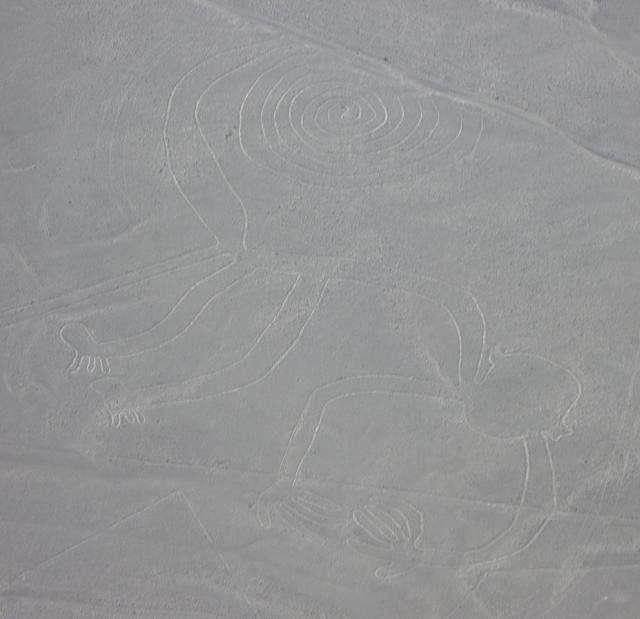
\includegraphics[width=4.8cm]{articles/Cote-du-sud/1255996049EeEt.jpg}
Singe à Nazca.

\hspace*{-0.65cm}
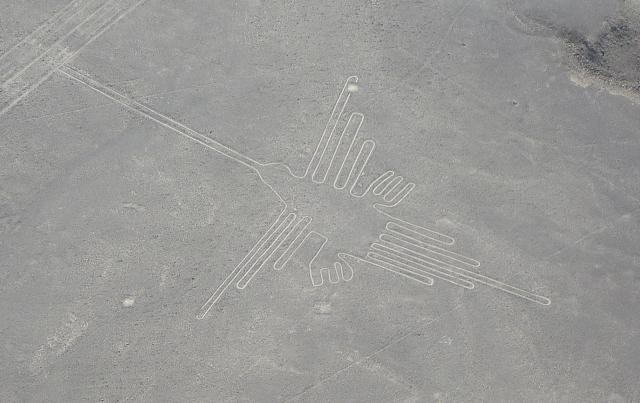
\includegraphics[width=4.8cm]{articles/Cote-du-sud/1255996046TE4T.jpg}
Colibri à Nazca.


En arrivant a Nazca, je rencontre Didier, un Belge bien sympa qui a pris 6 mois de break pour voyager en Amérique latine et en Australie.  Ne nous reverrons plusieurs fois à Nazca, puis prendrons le même bus pour Arequipa, après les différents problèmes énoncés ci-dessous.

L'après midi, après avoir survolé les lignes, je me ballade à l'extérieur de Nazca où je rencontre un groupe de jeunes qui jouent au volley, je me pose à côté puis leur demande de jouer avec eux. Il m'acceptent avec plaisir et nous passons rapidement de 4 joueurs à 10, on rit de partout et je reste toute l'apres midi.

\hspace*{-0.65cm}
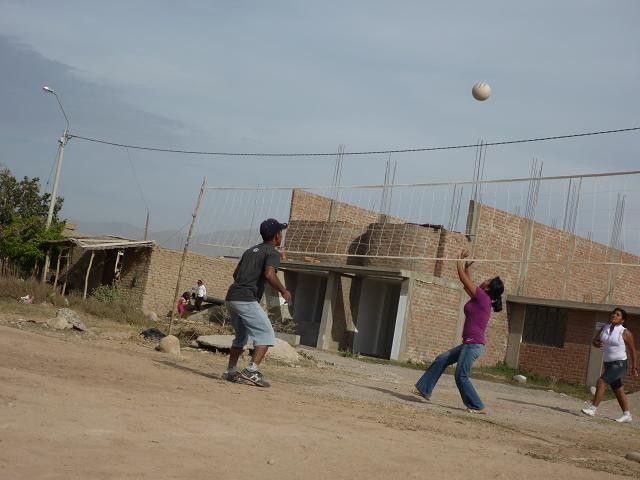
\includegraphics[width=4.8cm]{articles/Cote-du-sud/1255996043Enc7.jpg}
Après midi volley.


Plus tard, forcément, je leur demande si jeu peux dormir chez eux, ils acceptent avec grand enthousiasme, j'ai la baraka, le sourire jusqu'aux oreilles tellement je suis content de pouvoir faire ca. On se donne rendez vous à 21h sur la Plaza de Armas pour que je puisse aller décaler mon bus qui devait m'emmener à Arequipa cette nuit là. Je décale le bus, puis vais manger avec Didier et prend mon duvet pour aller au rendez vous. Personne ne viendra. J'attend une demi heure, puis prend la route en direction de l'endroit où nous avons fait du volley l'apres midi. Ce qui était simplement mal famé de jour devient ultra glauque de nuit. Des gardes de sécurité patrouillent avec armes et sifflets, ils sifflent a tout bout de champs, je me demande simplement comment il est possible de dormir avec le bruit qu'il font, accompagné des aboiement des chiens errants que je dérange apparement. Je ne retrouve pas la casa de mi amigos, je demande a un garde, il ne connait pas, forcément les seuls prénoms que j'ai a lui soumettre sont en fait des surnoms western pour leur adresse email. Puis le garde se souvient de m'avoir vu jouer au volley dans l'après midi, il m'indique où c'était et je revoit la maison. Les bonnes personnes ne sont plus là, ou elles se cachent, je ne sait pas. Ce que je comprend est que l'état d'esprit a changé depuis cet apres midi et que je suis redevenu un inconnu, je repars donc sans insister, et vais rechanger mon bus vu qu'il n'est pas trop tard. Oui, mais non.. Le bus a eu un problème en venant de Lima, il ne passera pas. On aura le suivant à 1h du mat' au lieu de 23h30. Pour Didier et moi ça ne change pas grand chose. On doit juste rendre notre billets pour en avoir un nouveau gratuit. Le problème est que je ne retrouve plus ce ticket, impossible d'en avoir un nouveau sans rendre l'ancien, et puis c'est 10 dollars US donc j'ai pas envie de repayer, la solution est d'aller faire une déclaration de perte au commissariat, la déclaration servira de billet d'échange. Et la commence le comique, le pittoresque. Allez faire bouger un flic pour avoir un bout de papier officiel de sa part au Pérou... et à minuit !! Il me demande nombre d'informations inutiles, il n'est pas allé jusqu'à l'âge de ma première dent, mais l'esprit y était. Puis monsieur le commissaire se met devant sa machine a écrire, met sont papier, le carbone, et le deuxième papier et commence son roman. Le plus marrant est quand il y a une faute d'orthographe il faut alors mettre du blanco sur une feuille, puis l'autre, puis réécrire sur l'une, puis l'autre (le carbone ne doit pas passer sur le blanco j'imagine...). Bref, une heure apres me voici avec mon sésame, tamponé 5 fois (ah les tampons, les flics et les douaniers aiment ça à peu près partout où je suis passé en voyageant). Je ne pourrais méme pas garder ce papier, j'ai dû le rendre contre un nouveau billet, dommage..

Voila, c'est la fin du recit pour aujourd'hui. Je suis actuellement à Arequipa avec Didier, dans le sud du Perou et nous partons cette nuit prendre un bus direction l'un des cañons les plus profonds du monde. Je prendrai ensuite la route direction la Bolivie et le Salaar de Uyuni, en passant sans doute par le Chili un ou deux jours. Le programme ensuite sera sans doute une remontée de la Bolivie par Sucre, Santa Cruz et La Paz, puis le lac Titicaca et le Machu Pichu, près de Cuzco.

Je vous dit à tous à très bientôt, et merci pour tous ces commentaires, c'est toujours très agréable de vous lire.

Muchas Besos, Etienne.

\end{multicols}

\bigskip
\textbf{\textsc{Commentaires}}

 \medskip
Tatid a écrit le 20 oct. 2009 :
\begin{displayquote}
Rahhh, j'suis deg, ton anti-spam a trop bien marché, il a vu que c'était faux (or c'était juste) et il m'a buté mon long message :-P !
Bref, je disais donc que je m'étonnais de ne pas avoir eu de news sur mon lecteur de flux RSS ! Je me disais que ton truc bugguait (comme l'anti-spam :p), et en fait non, je découvre aujourd'hui avec plaisir qu'il y a de tes nouvelles, donc je m'empresse de les lire !
En tous cas, tu me fais bien rire, le dud-voyageur n'a pas changé d'un poil, toujours le même, toujours à l'arrache sans aucun stress ! C'est quand même génial ce que tu vis ! Profite bien des rencontres, c'est le mieux dans un voyage : la richesse humaine ;-))
Keep us posted, and say "hey" to the American familly for me... See, americans are not all stupid haha!
\end{displayquote}

 \medskip
Titou et Chachou a écrit le 20 oct. 2009 :
\begin{displayquote}
Salut le voyageur,
Comme le dit Tatid, content d'avoir de tes nouvelles, on s'inquiétait un piti peu :p
Tu as l'air de bien en profiter malgré tes quelques mésaventures avec la police Sud-américaine. En même temps, ce serait pas arrivé si tu avais une tête ;-) C'est du toi tout craché.
Continue d'en profiter et tu peux même éviter les endroits glauques si tu veux... Si tu veux qu'ils t'invitent à dormir plus facilement, pense au poncho et au bonnet pour te fondre dans la masse :p
Fais bien gaffe à toi et tiens nous au courant.
Bisous
\end{displayquote}

 \medskip
Zé a écrit le 23 oct. 2009 :
\begin{displayquote}
Buenas Etienne, qué màs...
Lo pasas bien creo, pues disfruta!!!
Me gustaron las fotos, y me imagino que tendràs muchas cosas que contarme...
Ojalà pudiera visitar contigo estas tierras que tanto me fascinan.
Seguimos jugando al fùtbol los domingos por la mañana, quizà vengas algùn dìa rolar la pelota con nosostros...
Seguiré visitando tu pàgina para aprovechar tus aventuras!
Hasta luego, abrazo.
\end{displayquote}

 \medskip
Titou et Chachou a écrit le 28 oct. 2009 :
\begin{displayquote}
Salut ti Dud,
bon ba c'est pas que ça fait longtemps qu'on a pas eu de news de ta part mais quand même !!! On espère que tout va bien et que tu profites bien de ton séjour !
Grosse léchouille et on espère à très vite !
\end{displayquote}

 \medskip
Salah Eddine a écrit le 01 nov. 2009 :
\begin{displayquote}
Holla chico,

Espero que la vida en America del sur te gusta commo la imaginabas despues de partir. Pues, si si senor, hablo espanol muy bien, pero nunca he tenido suerte para ir a visitar las paises espanophones. Espero que la proxima ves, puedas invitarme a viajar contigo.

Bref, mec, la grande découverte, c'est que les keufs là bas sont pires que les marocains. T'aurais du essayé de graissé la patte :). Je sais pas si ça marche là bas. c'est malhonnête en même temps. Mais c clair que vous aviez du vous marrer. T'aurais du prendre le poste en photo, j'aurais bien aimé voir sa tronche au flic :).

Franchement, super belle aventure. Bonne continuation.

A+ !
\end{displayquote}


